\section{CutMax a new approximate mathing algorithm}
\label{section:our}

In the section we present several algorithms for approximate pattern mathing that heavily based on semi-local sequence alignment and it's underlying algebraic structure.
The presented algorithms also support length constraints on the result (on detected clones).

The first algorithm~\ref{alg:appximateMatchingGreedy} implements an idea of the greedy choice of the most suitable clone on each step, i.e. it looks for the most similar substring with length in interval $[\alpha,\ \beta]$ each time for some predefined constants $\alpha$ and $\beta$.
In other words, it constructs a non-intersected set $\Tau$ of clones of pattern $p$ in text $t$ such that on each step it adds $\tau_i$ to $\Tau$ iff $\tau_i$ has the highest similarity score with $p$ in the rest of the text and its length satisies the length constraint, i.e. $\alpha \leq |\tau_i| \leq \beta$.
%% The first algorithm~\ref{alg:appximateMatchingGreedy} refers to following constraint.
%% There should be found all non-intersected clones $\tau_{i}$ of pattern $p$ from text $t$ that has the highest similarity score on the uncovered part of the text $t$ and $\alpha \geq |\tau_{i}| \geq \beta$  i.e algorithm should perform greedy choice at each step with length constraint on $\tau_{i}$.
%% This is a more intuitive approach i.e like looking for the most similar substring every time with length at least $l$ and at most $r$.
Formally:\todo{check l and r}
\begin{equation}
   \Tau = \bigcup_{i} \tau_i = \bigcup_i \argmax_{l,r \in (t \cap (\cup_{j=1}^{i-1} \tau_{j}),l<r, \alpha \leq |t_{l,r}| \leq \beta ,t_{l,r} \cap (\cup_{j=1}^{i-1} \tau_{j}) = \emptyset } sa(t_{l,r}, p)
\end{equation}

The algorithm proceeds as follows.

First, the semi-local sa problem is solved for given pattern $p$ and text $t$ (line 1).
Then, the solution for the string-substring subproblem is queried from it (lines 2--3).
Further, the diagonal slice of width $\beta-\alpha$ which corresponds to scores of substrings of size in $[\alpha,\ \beta]$ is cropped to get a partial Monge matrix (line 4) (\ref{figures:M2}).
\todo{Upon partial matrix $M_{partial}$, the full Monge Matrix $M$ is built to build \emph{rmq2D} data structure  for performing range minimum queries on $M$ by Theorem \ref{partialTheorem}.}



\begin{figure}[H]
	\centering
    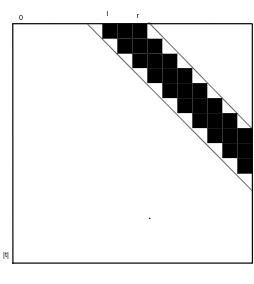
\includegraphics[width=0.4\columnwidth]{figures/M1.png}
    \caption{Диагfрамма компонентов системы}\label{figures:M2}
\end{figure}

Then, algorithm calls recursive subroutine $greedy$ (algorithm \ref{alg:rec}).
The $greedy$ routine performs greedy choice of $\tau_{k}$ with maximal alignment within a continious uncovered part of the text $t_{i,j}$ with length boundaries for $\tau_{k}$ in $[\alpha:\beta]$ where $t_{i,j}$ denotes a substing of text $t$ starting at $i$-th element and ending at $j$-th element.
More precisely, it refers to searching maximum value with corresponding position (row and column) in matrix $M$ within $t_{i,j}$.
The search is performed via range queries.
When detected $interval$ has alignment score less then threshold it means that no clones of pattern $p$ are presented in this part of text $t_{i,j}$, and further processing should be skipped.
Otherwise, the founded clone $\tau_k$ is added to the final result and the current part of the text splits into two smaller parts and processed recursively in the same way.

Finally, the algorithm outputs a set of the non-intersected intervals of clones of pattern $p$ in text $t$.


\begin{algorithm}[H]
\caption{Greedy subroutine}
\label{alg:rec}
Input: $rmq2D$--- range maximum query data structure for performing range queries on Monge matrix $M$, $h$ --- threshold value, $i,j$ --- start and end positions of current text $t_{i,j}$, $l,r$--- length boundaries for detected intervals \\
Output: Set of non-intersected intervals from $t_{i,j}$\\
Pseudocode:\\
$greedy(rmq2D,h, i, j, t_{i,j},l,r ):$

\begin{algorithmic}[1]
\STATE{$interval = rmq2D.query(i,j,i,j)$}
\STATE{$result = \emptyset$}
\IF{ $interval.score < h $}
\RETURN $result$
\ENDIF
\IF{ $interval.i - i \geq l $}
\STATE{$cl = greedy(rmq2D,h,i,interval.i,t_{i,interval.i},l,r)$}
\STATE{$result.add(cl)$}
\ENDIF
\IF{$j - interval.j \geq l$}
\STATE{$cl = greedy(rmq2D,h,j,interval.j,t_{j,interval.j},l,r)$}
\STATE{$result.add(cl)$}
\ENDIF
\RETURN $result$
\end{algorithmic}
\end{algorithm}


\begin{algorithm}[H]
\caption{GREEDY-PATTERN BASED NEAR DUPLICATE
SEARCH ALGORITHM}
\label{alg:appximateMatchingGreedy}
Input: pattern $p$ and text $t$, threshold value $h$\\
Output: Set of non-intersected clones of pattern $p$ in text $t$\\
Pseudocode:\\
$GreedyMathing(M,h,t)$
\begin{algorithmic}[1]
\STATE{$sa = semilocalsa(a,b)$}
\COMMENT{1st phase}
\STATE{$H = sa.getAssociatedMatrix()$}
\STATE{$H^{str-sub} = H.stringSubstringMatrix()$}
\STATE{$M_{partial} = -getPartialMatrix(H^{str-sub},l,r)$}
\COMMENT{2nd phase}
\STATE{$M = builtMongeMatrix(M_{partial})$}

\STATE{$rmq2D = buildRMQStructure(M) $}
\STATE{$result = greedy(rmq2D,h,0,|t|,t,l,r)$}
\COMMENT{3rd phase}
\RETURN $result$
\end{algorithmic}
\end{algorithm}


\begin{theorem}
Algorithm \ref{alg:appximateMatchingGreedy} could  be solved in
$O(max(|t||p|,\frac{|t| \log^2 |t|}{\log \log |t|} ))$ time and $O(|t| )$ space when $|p|<|t|$ where $p$ is pattern, $t$, is text and $v=O(1)$ is denominator of normalized mismatch score for semi-local sequence alignment
$w_{normalized} = (1,\frac{\mu}{v},0)$.
\end{theorem}
Note that $|p|<|t|$ and $v=O(1)$.
For simplicity let $v=1$ (same true for other $v=O(1)$).

\emph{First phase}. 
We need to solve $semi-local lcs$ because $v=1$.
It could be solved implicitly via algorithm from \cite{.}
in $O(|t||p|)$ with $O(|t|)$ additional space when $O(|p|<|t|)$
Note that we only interesting in string-substring submatrix $H^{str-sub}_{p,t}$ of size $|t| \times |t|$.
Upon associated permutation matrix with $H^{str-sub}_{p,t}$ anti-Monge matrix ( Theorem \ref{decomposition})  we build data structure
of size $O(|t|)$ in $O(|t|\sqrt{\log(|t|))}$ time to 
perform  orthogonal range queries in $O(\frac{\log (|t|)}{\log \log (|t|)})$ time.

Thus, the overall time and space complexity of first phase 
is $max(O(|t|  \sqrt{\log(|t|))},O(|p||t|))$ and
$O(|t|)$ respectively.

\emph{Second phase}.
In string-substring matrix $H^{str-sub}_{p,t}$ we only interesting in diagonal of length $r-l$ that refers to all substrings of text $t$ with length in $[l:r]$ interval. 
If we apply to  $H^{str-sub}_{p,t}$ inverse operation and cut this diagonal we will have partial Monge matrix $M_{partial}$.
Then we apply theorem  \ref{partialTheorem} to build 
\emph{rmq2D} data structure to perform minimum range queries.
Note that we have non-constant access to the element in $M_{partial}$ and we will return not the element itself but also associated indices of it.
Thus, the data structure of size 
$O(|t|)$
 can be built in $O(|t| \log |t|)* O(\frac{\log (|t|)}{\log \log (|t|)}) = O(\frac{|t|\log^2 |t|}{\log \log (|t|)}) $ time
to perform range minimum queries in $O(\log \log (|t|))*O(\frac{\log (|t|)}{\log \log (|t|)})=O(\log |t|)$ time.

Then, overall time and space complexity of second phase is 
$O(|t| \log^2 |t|)$ and
$O(|t|)$
respectively.


\emph{Third phase}

To analyze the third phase we need to look at the recursive algorithm \ref{alg:rec}.
Note that at the worst case we will have $O(|t|)$ nodes while proceeded recursion due to fact that at the worst case on each node we will detect interval of size 1.
Such non-intersected intervals will be at most $t$.
Thus, the total amount of calls to $query$ operation will be at most 
$O(|t|)$.
The query operation requires $O(\log |t|)$ as shown in the previous phase.
Thus, the total running time and space complexity of third phase is 
$O(|t| |\log t|)$ and $O(|t|)$  

Then, overall algorithm running time and space complexity is as claimed when $v=O(1)$ and $|p|<|t|$.




The second algorithm \ref{alg:appximateMatchingMax} uses a less sophisticated approach but found fewer duplicates of pattern $p$.
It also uses length constraint but greedy approach
is much simpler.

\paragraph{Algorithm description}

The first phase as in \ref{alg:appximateMatchingGreedy}
On the second phase we use Lemma \ref{lemma} to implicitly fill 
elements of partial Monge matrix to get $M$ Monge matrix.
Then we solve the following problem (Line 6).
For each prefix of text $t$ we find the suffix that has the highest similarity score with pattern $p$:
$$ a[j] = \max _{i \in 0 ..j} sa(p,t[i,j]), j \in 0..|t|$$

Further, we remove suffixes whose similarity is below the given threshold of $h$ (Line 4).
Then remaining suffixes are sorted in descending order (Line 5) and the interval tree is built upon them (Lines 9-14).
The building process consists of checking that current substring $candidate$ not intersected with already added substrings to $tree$ and adding it to $tree$.
Finally, algorithm output set of non-intersected substrings (clones) of pattern $p$ in text $t$.


\begin{algorithm}[H]
\caption{Greedy approximate}
\label{alg:appximateMatchingMax}
Input: pattern $p$, text $t$, threshold value $h$\\
Output: Set of non-intersected clones of pattern $p$ in text $t$\\
Pseudocode:
\begin{algorithmic}[1]

\STATE{$sa = semilocalsa(p,t)$}
\COMMENT{1st phase}
\STATE{$H = sa.getAssociatedMatrix()$}
\STATE{$H^{str-sub} = H.stringSubstringMatrix()$}
\STATE{$M_{partial} = -getPartialMatrix(H^{str-sub},l,r)$}
\STATE{$M = fillToMongeMatrix(M_{partial})$ }
\COMMENT{2nd phase}
\STATE{$colmax = smawk(M) $}
\STATE{$colmax.filter(it.score >= h$)}
\STATE{$colmax.sortByDescending(it.score)$}
\STATE{$tree = buildIntervalTree()$}
\FOR{$candidate \in colmax$}
%\COMMENT{3rd phase}
\IF{$candidate \cap tree = \emptyset $}
\STATE{$tree.add(candidate)$}
\ENDIF
\ENDFOR
\STATE{$result = tree.toList()$}
\RETURN $result$
\end{algorithmic}
\end{algorithm}

\begin{theorem}
Algorithm \ref{alg:appximateMatchingMax} could  be solved in
$\max (O(|p||t|), O(|t|* \log |t|))$ time with $O(|t|  \log {|t| * v })$ space when $|p|<|t|$ where $p$ is pattern, $t$ is text and $v=O(1)$ is denominator of normalized mismatch score for semi-local sequence alignment
$w_{normalized} = (1,\frac{\mu}{v},0)$.
\end{theorem}

\emph{First phase}.
The total running time and space complexity of first phase is 
$max(O(|t||p|, |t| \log |t|)$ as in \ref{alg:appximateMatchingGreedy}.


At the second phase we use Lemma \ref{lemma} with non-constant access to matrix element of $O(\frac{\log |t|}{\log \log |t|})$.
Then, running time complexity of implicitly filling
blank entries in $M_{partial}$ is 
$O(\frac{|t| \log |t|}{\log \log |t|})$ to get Monge matrix $M$.
Then to find for each prefix the suffix that is most similar to pattern $p$ with length in $[l:r]$ we simply run \emph{SMAWK}
the algorithm on matrix $M$ (Line 6).
After that we will filter out resulting suffices by given threshold $h$ and sort remaining suffices in descending order (Lines 7-8).
There will be at most $O(r-l)=O(|t| - 0) = O(|t|)$ suffices.
Thus sort operation complexity  is $O(|t| \log |t|)$.

\emph{Third phase}
$Colmax$ array has as worst-case $O(|t|)$ elements when filtering does not eliminate any substrings.
Thus, 
there are at most $O(|t|)$ additions and intersections with the tree (Lines 11-12).
Since both operation time complexity is  $O(\log |t|)$.
Then overall running time complexity is $O(|t|\log |t|)$.

Thereby, the total time and space complexity of algorithm is $\max (O(|p|*|t|), O(|t|* \log |t| ))$ and $O(|t|)$  respectively.
 

\begin{corollary}
Algorithm \ref{alg:appximateMatchingMax} could  be solved in 
$O(|p| * |t|)$.
\end{corollary}

When the amount of clones is relatively small and the threshold value $h$ is set high,  then after filtering out $t$ intervals (Line 4) sorting is performed on s small set of elements.
Thus, this part is dominated by calculating semi-local sa solution.







  

%Given some rope $t$ and small rope $p$ you need to make cuts to form small ropes $t_{i_{1},j_{1}},t_{i_{2},j_{2}}...,t_{i_{k},j_{k}}$ for some $k$ and select some of them that very similiar to  rope $p$ i.e have high similiarity score.
%For that, we would consider constarint that each select of $t_{k} = t_{i_{k},j_{k}}$ should be made greedy i.e   $t_{k}$ it has the highest similiarity score against $p$ over all possible choices of      

 
%The following interpretation can be applied.
%Given text interval $t_{i}$   
